\section{Implementation}

The mining pool is written in Django, a web framework for Python which allows for very rapid development. With Django we could focus on the practical side rather than solving unrelated technical difficulties. \\

The mining pool is very lightweight and only spans around 500 lines of code. It consists of two HTTP routes, one for \texttt{/} which miners use, and \texttt{/info} which is a web interface showing pool status. The routes are stored in \texttt{urls.py} and their corresponding endpoints in \texttt{views.py}. Furthermore we wrote two custom classes. The first is \texttt{Block} in \texttt{block.py} for constructing the block, templates and converting various hexadecimal values. The second is \texttt{RPC} in \texttt{rpc.py} for communicating with the wallet. \\

The mining pool uses an SQLite database to store the shares submitted by miners. Its structure is found in \texttt{models.py}, it stores the share timestamp, address of the miner, height of the block, difficulty of the submission and the actual difficulty required by the wallet. \\

The miner starts by sending a POST request to \texttt{/} with the \texttt{getblocktemplate} command. The server then asks the wallet for the current block template, uses that information to construct a \texttt{Block} instance with the same data but a custom coinbase and a much lower difficulty. \\

When the miner has found a solution it sends a POST request to \texttt{/} with the \texttt{submitblock} command. The server then calculates the difficulty of that submission and if it matches or exceeds the network difficulty, the server uses the \texttt{RPC} class to send a \texttt{submitblock} to the wallet, thus successfully mining the block. If the submission difficulty is too low nothing happens, but information about the submission is stored in the \texttt{Shares} SQL table.

\subsection{Using the Mining Pool}

More detailed installation instructions can be found on GitHub. \\

The server can be started with the following command.

\begin{minted}[fontsize=\footnotesize]{text}
$ python manage.py runserver 0.0.0.0:8000
Watching for file changes with StatReloader
Performing system checks...

System check identified no issues (0 silenced).
December 14, 2019 - 02:51:36
Django version 2.2.7, using settings 'smlypool.settings'
Starting development server at http://0.0.0.0:8000/
Quit the server with CONTROL-C.
\end{minted}

The information web page is then available at \texttt{http://localhost:8000/info}. \\

We use an ASIC miner called FutureBit Moonlander 2 to test the mining pool. It comes with a custom build of \texttt{bfgminer}, a popular mining client. We start the miner with the following command, where we pass our payout address as username.

\begin{minted}[fontsize=\footnotesize]{text}
$ bfgminer --scrypt -o http://localhost:8000 -u BEppJqTLw5ByePPbZwm7hByqqwcmsCtVfK -p y -S ALL \
    --set MLD:clock=600 --no-getwork --no-stratum
\end{minted}

The miner should start blinking and soon it outputs something like this.

\begin{minted}[fontsize=\footnotesize]{text}
[2019-12-14 02:50:26] Accepted 000ec771 MLD 0  Diff 67m/10m
[2019-12-14 02:50:34] Accepted 0041d12a MLD 0  Diff 15m/10m
[2019-12-14 02:50:37] Accepted 0038248a MLD 0  Diff 17m/10m
[2019-12-14 02:50:37] Accepted 003ffc0a MLD 0  Diff 15m/10m
\end{minted}

This means that it has found solutions to its shares and is submitting them to the server. We can see these shares in the web interface as well.

\begin{table}[H]
\centering
\small
\begin{tabular}{|l|l|l|l|l|}
\hline
Time                     & Height & Miner                              & Submitted & Actual  \\ \hline
Dec. 14, 2019, 2:50 a.m. & 608802 & BEppJqTLw5ByePPbZwm7hByqqwcmsCtVfK & 0.0156    & 30.6154 \\ \hline
Dec. 14, 2019, 2:50 a.m. & 608802 & BEppJqTLw5ByePPbZwm7hByqqwcmsCtVfK & 0.0178    & 30.6154 \\ \hline
Dec. 14, 2019, 2:50 a.m. & 608802 & BEppJqTLw5ByePPbZwm7hByqqwcmsCtVfK & 0.0152    & 30.6154 \\ \hline
Dec. 14, 2019, 2:50 a.m. & 608802 & BEppJqTLw5ByePPbZwm7hByqqwcmsCtVfK & 0.0677    & 30.6154 \\ \hline
\end{tabular}
\caption{Shares as they appear on the information web page.}
\end{table}

As we can see the submitted difficulty is much lower than what is needed for the network. 

\subsection{Results}

After running the pool for around 12 hours, the miners had submitted 2691 blocks. The server is configured such that the difficulty for miners is 0.01, while the scrypt difficulty on the SmileyCoin network is usually around 10. The graph below shows the distribution of the submission difficulty. Most of the shares, $1295$ of them, were in the range $[0.01, 0.02]$. Then there were $460$ shares in the range $[0.02,0.03]$, and so on.

\begin{figure}[h]
    \centering
    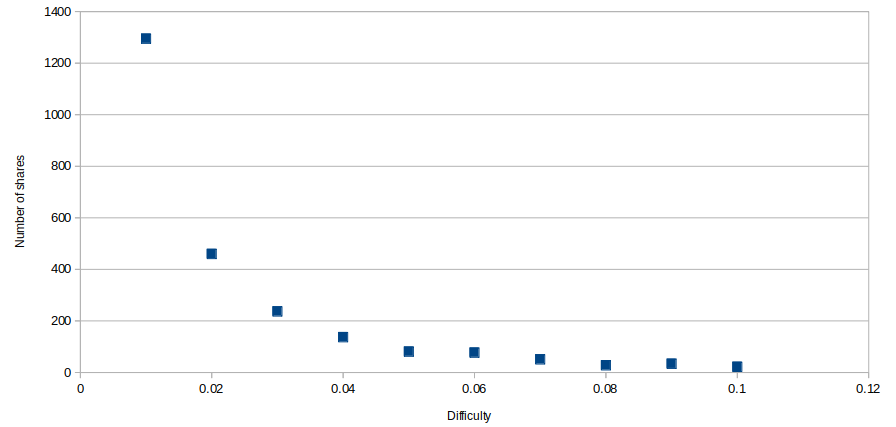
\includegraphics[width=0.9\textwidth]{difficulty_chart.png}
    \caption{Distribution of share difficulty}
\end{figure}

During the time we ran the pool, difficulty for scrypt was unusually high (around 30 to 40) so we were unable to find any solutions. We had hoped to submit a block to the blockchain with a custom coinbase as a proof of concept. The block submissions have been confirmed to pass the \texttt{CheckBlock()} function in the wallet. The coinbase are also confirmed to be valid, as can be seen on the next page.

\subsubsection{Example of Custom Coinbase}

\begin{minted}[fontsize=\scriptsize]{text}
 smly decoderawtransaction 01000000010000000000000000000000000000000000000000000000000000000000000000ffffffff16032
 c4b09030d25090103062f42534d4c59504f4684dfffffffff0500743ba40b0000001976a91471cda15b815ec0411c1c74412598d9e695c6e3
 7988ac00ac23fc060000001976a9141120acffc8b30a852913dd420fc19ca6f1b770f988ac00c817a8040000001976a9142cab003c8b268c8
 15688b9eed6cfc477997b366f88ac001417c6680000001976a914e8dbc5ac7e84cea890b29c2dcc74a5391adc225c88ac001417c668000000
 1976a914db7aeaa2443fb3c91662392c6cac2f6eb8f0ef6e88ac00000000

    ...
    "vout" : [
        {
            "value" : 500.00000000,
            "n" : 0,
            "scriptPubKey" : {
                "asm" : "OP_DUP OP_HASH160 71cda15b815ec0411c1c74412598d9e695c6e379 OP_EQUALVERIFY OP_CHECKSIG",
                "hex" : "76a91471cda15b815ec0411c1c74412598d9e695c6e37988ac",
                "reqSigs" : 1,
                "type" : "pubkeyhash",
                "addresses" : [
                    "BEppJqTLw5ByePPbZwm7hByqqwcmsCtVfK"
                ]
            }
        },
        {
            "value" : 300.00000000,
            "n" : 1,
            "scriptPubKey" : {
                "asm" : "OP_DUP OP_HASH160 1120acffc8b30a852913dd420fc19ca6f1b770f9 OP_EQUALVERIFY OP_CHECKSIG",
                "hex" : "76a9141120acffc8b30a852913dd420fc19ca6f1b770f988ac",
                "reqSigs" : 1,
                "type" : "pubkeyhash",
                "addresses" : [
                    "B61eFL4bvYznW1UEXJgHcESHD588wyAfR7"
                ]
            }
        },
        {
            "value" : 200.00000000,
            "n" : 2,
            "scriptPubKey" : {
                "asm" : "OP_DUP OP_HASH160 2cab003c8b268c815688b9eed6cfc477997b366f OP_EQUALVERIFY OP_CHECKSIG",
                "hex" : "76a9142cab003c8b268c815688b9eed6cfc477997b366f88ac",
                "reqSigs" : 1,
                "type" : "pubkeyhash",
                "addresses" : [
                    "B8XGCWSvQUKGbXRF9ScWsFp7nMTqq6P7zM"
                ]
            }
        },
        {
            "value" : 4500.00000000,
            "n" : 3,
            "scriptPubKey" : {
                "asm" : "OP_DUP OP_HASH160 e8dbc5ac7e84cea890b29c2dcc74a5391adc225c OP_EQUALVERIFY OP_CHECKSIG",
                "hex" : "76a914e8dbc5ac7e84cea890b29c2dcc74a5391adc225c88ac",
                "reqSigs" : 1,
                "type" : "pubkeyhash",
                "addresses" : [
                    "BRgKfFuPEVFHNKWUfSnobX2byUVmUMVhux"
                ]
            }
        },
        {
            "value" : 4500.00000000,
            "n" : 4,
            "scriptPubKey" : {
                "asm" : "OP_DUP OP_HASH160 db7aeaa2443fb3c91662392c6cac2f6eb8f0ef6e OP_EQUALVERIFY OP_CHECKSIG",
                "hex" : "76a914db7aeaa2443fb3c91662392c6cac2f6eb8f0ef6e88ac",
\end{minted}

\newpage

\subsection{Code Reference}

\subsubsection{class block.Block()}

This class contains the structure of the current block and includes methods to construct block templates. \\

\texttt{create\_coinbase(outputs)} \\

Builds the coinbase for the block, outputs is a dictionary of addresses and corresponding shares, the shares will be normalized such that the total outputs equal 1000 SMLY. \\

\texttt{create\_gbt(difficulty)} \\

Constructs the \texttt{getblocktemplate} response for miners with the requested difficulty. \\

\texttt{get\_submission\_difficulty(block\_hex)} \\

Calculates the difficulty of the hash of a raw block submission. When miners use submitblock this is used to calculate the difficulty. \\

\texttt{target\_to\_difficulty(target)}\\

Convert the header target field into a difficulty integer. \\

\texttt{difficulty\_to\_target\_hash(difficulty)}\\

Convert difficulty int to a hash target for block template. \\

\subsubsection{class rpc.RPC()}

This class is used to communicate with the SmileyCoin wallet. \\

\texttt{call(cmd, [params])}\\

Sends a command to the wallet with optional parameters and returns the response.
